\section{Analyse des données}

\begin{frame}
  \frtt{Analyse des données}
	\begin{itemize}
	  \item L'équation des moindres carrés:
      \item $X(t) + i \times Y(t) = \sum\limits_{j=1}^{40} (\widetilde{A}_{j} \times e^{(\omega_{j}*t + \varphi_{j})})$
      \item $\widetilde{A} = A_{Re} + i \times A_{Im}$
	\end{itemize}
\end{frame}

\begin{frame}
  \frtt{Changement de dX et dY à la basé de la fréquence}
	\begin{center}
		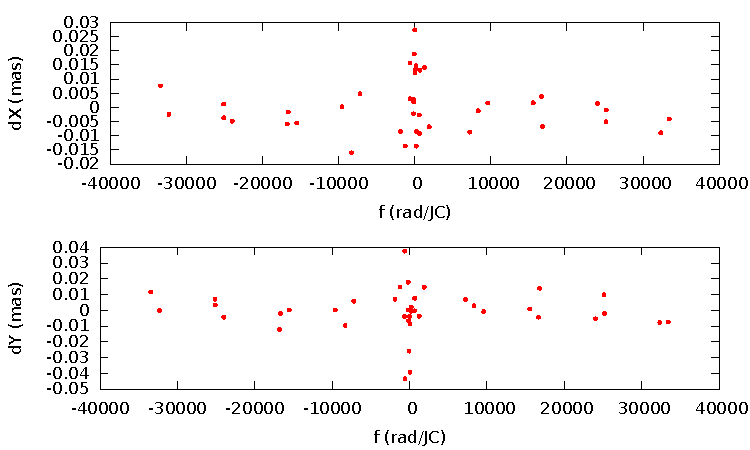
\includegraphics[width=1.0\textwidth]{amplitude_freq.pdf}
	\end{center}
\end{frame}

\begin{frame}
  \frtt{Comparaison de dX et dY entre la série et de l'observation}
	\begin{center}
		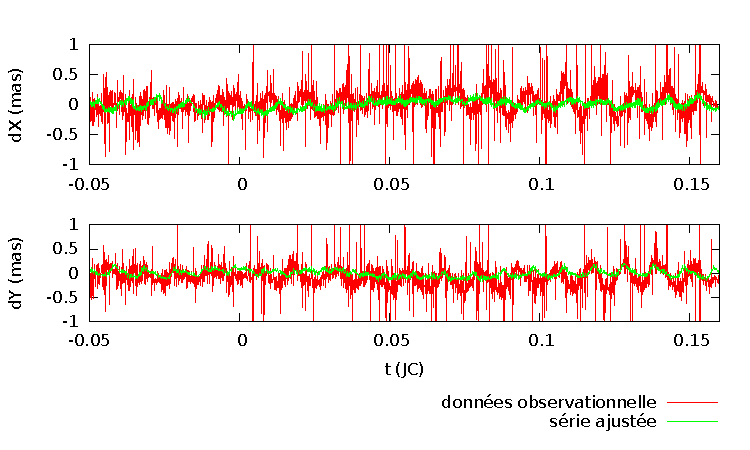
\includegraphics[width=1.0\textwidth]{fit_amplitude_ser_obs.pdf}
	\end{center}
\end{frame}

\begin{frame}
	\begin{center}
		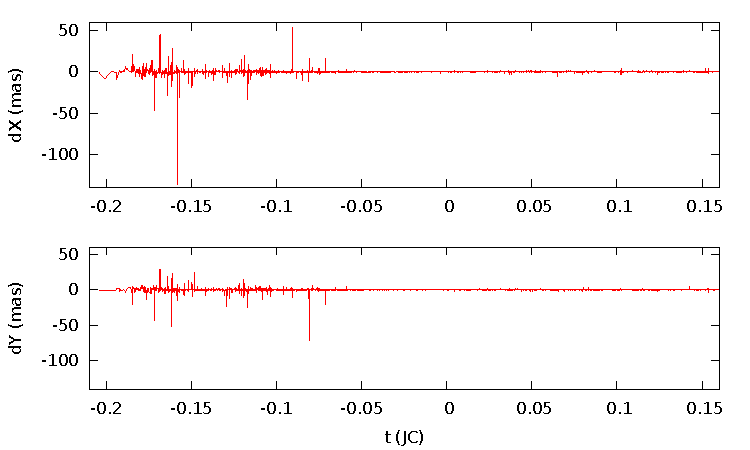
\includegraphics[width=1.0\textwidth]{fit_amplitude_obs-ser.pdf}
	\end{center}
\end{frame}